\documentclass{article}
\usepackage[letterpaper,margin=1cm,landscape]{geometry}
\usepackage{tikz}
\usetikzlibrary{shapes.geometric, arrows}
\begin{document}
\thispagestyle{empty}
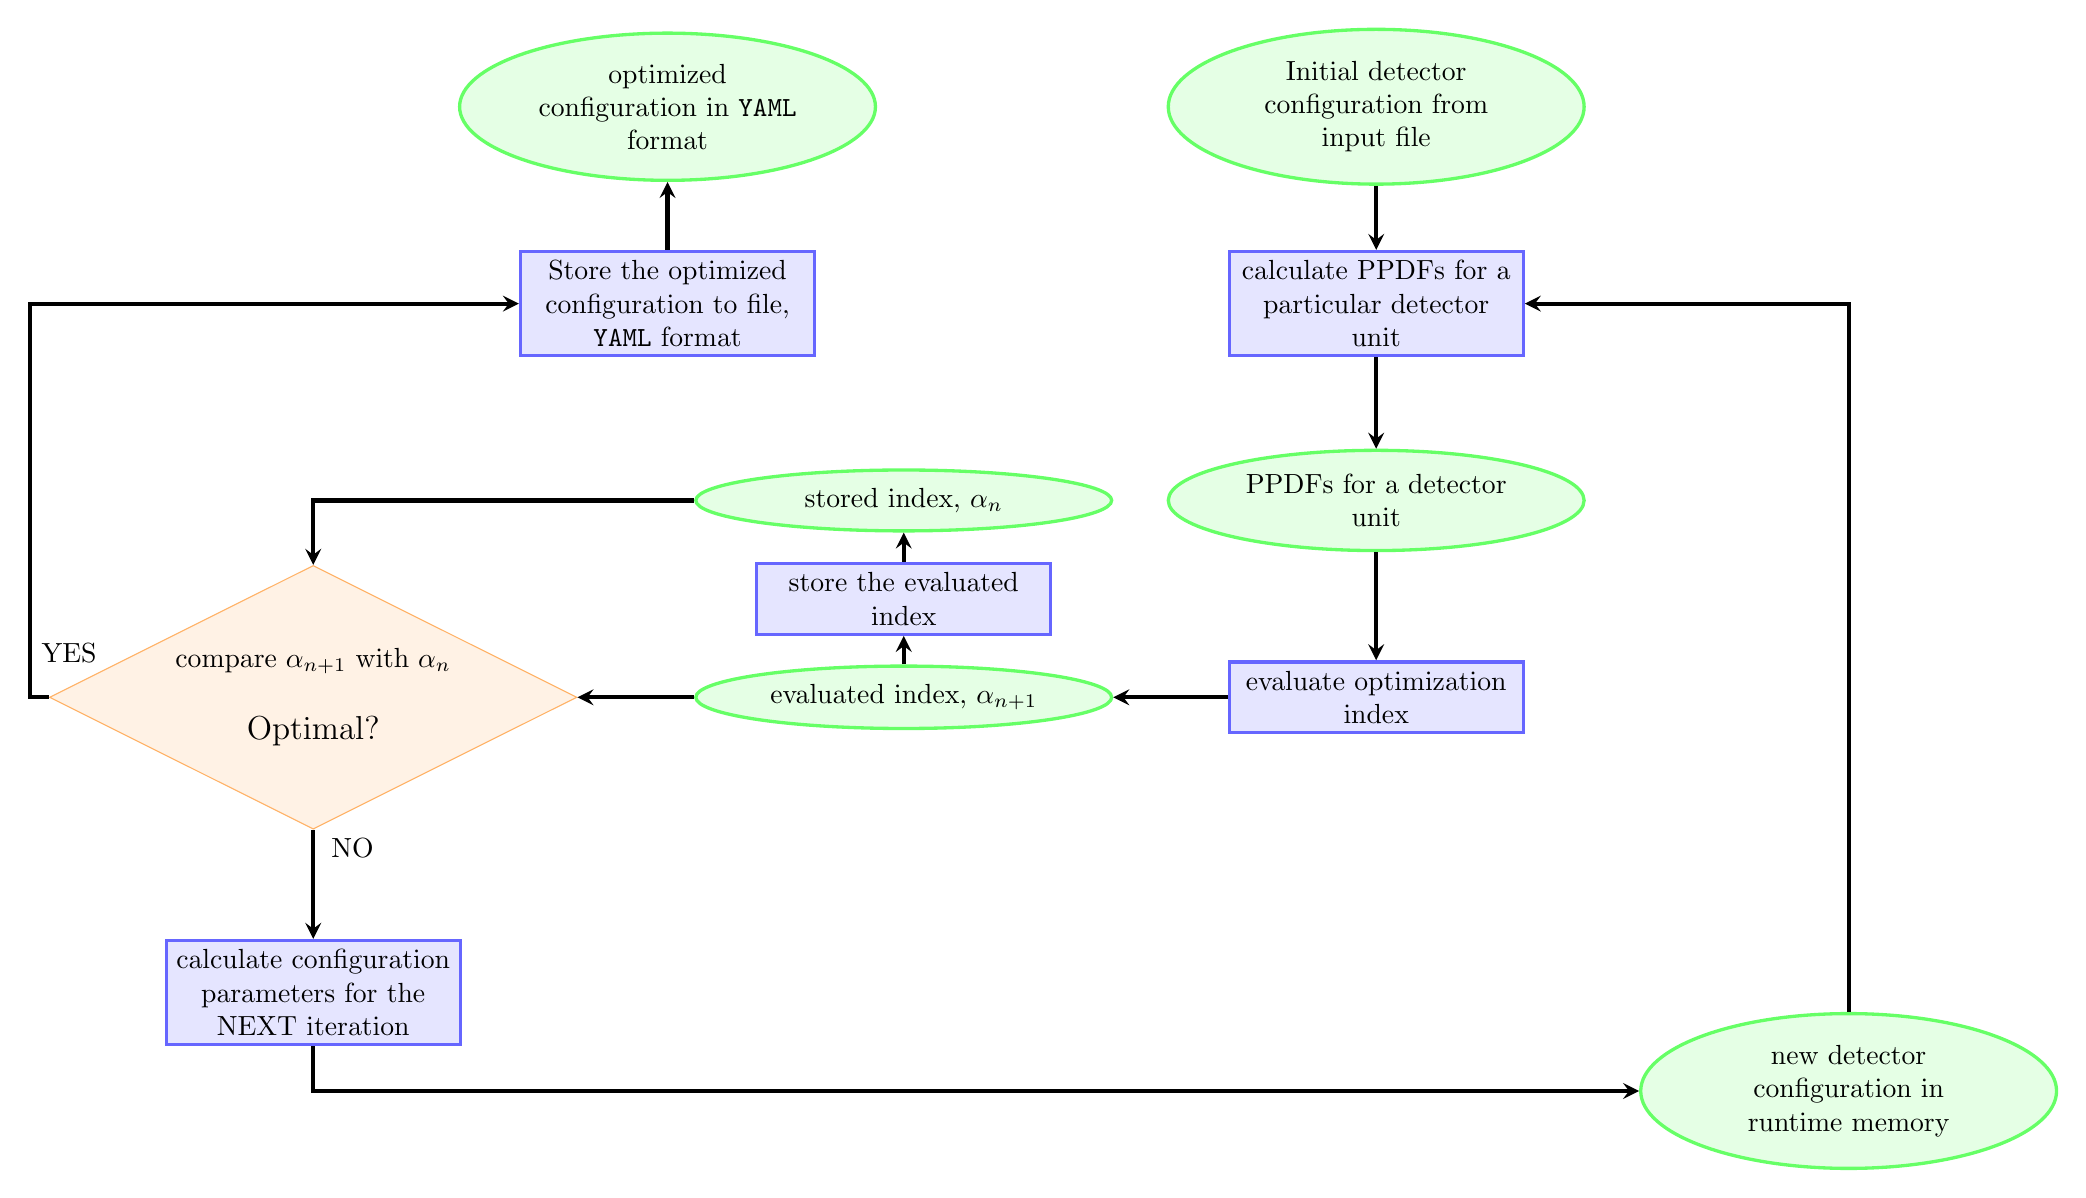
\begin{tikzpicture}[
        roundnode/.style={ellipse, draw=green!60, fill=green!10, very thick, minimum width=5mm, align=flush center, text width=3.5cm},
        squarednode/.style={rectangle, draw=blue!60, fill=blue!10, very thick, minimum size=5mm,align=flush center, text width=3.5cm},
        decisionnode/.style={draw, diamond,aspect=2,align=flush center, text width=3.5cm,draw=orange!60, fill=orange!10},
        arrow/.style = {thick,->,>=stealth, line width=1.5pt},
        x=3cm,y=2.5cm,
    ]
    \node[roundnode] (0) at (0,0) {Initial detector configuration from input file};
    \node[squarednode] (1) at (0,-1) {calculate PPDFs for a particular detector unit};
    \node[roundnode] (2) at (0,-2) {PPDFs for a detector unit};
    \node[squarednode] (3) at (0,-3) {evaluate optimization index};
    \node[roundnode] (5) at (2,-5) {new detector configuration in runtime memory};
    \node[roundnode] (6) at (-2,-3) {evaluated index, $\alpha_{n+1}$};
    \node[squarednode] (7) at (-2,-2.5) {store the evaluated index};
    \node[roundnode] (8) at (-2,-2) {stored index, $\alpha_n$};
    \node[decisionnode] (9) at (-4.5,-3) {compare $\alpha_{n+1}$ with $\alpha_{n}$\\\vspace*{0.5cm} {\large Optimal?}};
    \node[squarednode] (10) at (-4.5, -4.5) {calculate configuration parameters for the NEXT iteration};
    \node[squarednode] (4) at (-3, -1) {Store the optimized configuration to file, \texttt{YAML} format};
    \node[roundnode] (11) at (-3, 0) {optimized configuration in \texttt{YAML} format};
    \draw [arrow] (0) -- (1);
    \draw [arrow] (1) -- (2);
    \draw [arrow] (2) -- (3);
    \draw [arrow] (5) |- (1);
    \draw [arrow] (3) -- (6);
    \draw [arrow] (6) -- (7);
    \draw [arrow] (7) -- (8);
    \draw [arrow] (8) -- (-4.5,-2) -- (9);
    \draw [arrow] (6) -- (9);
    \draw [arrow] (9) -- node[right=0.5cm,above=0.2cm]{NO}(10);
    \draw [arrow] (10) |- (5);
    \draw [arrow] (9) -| node[right=0.5cm,above=0.3cm]{YES}(-5.7,-1) -- (4);
    \draw [arrow] (4) -- (11);
\end{tikzpicture}
\end{document}